%% LyX 2.0.5.1 created this file.  For more info, see http://www.lyx.org/.
%% Do not edit unless you really know what you are doing.
%\documentclass[12pt,english]{report}
%\usepackage{mathptmx}
%\renewcommand{\familydefault}{\rmdefault}
%\usepackage[T1]{fontenc}
%\usepackage[latin9]{inputenc}
%\usepackage[a4paper]{geometry}
%\setcounter{secnumdepth}{2} % Changed from 3 to 2. 0-chapter 1-section 2-subsection 
%\setcounter{tocdepth}{2} % Changed from 3 to 2. 0-chapter 1-section 2-subsection 
%\setlength{\parskip}{\medskipamount}
%\setlength{\parindent}{0pt}
%\usepackage{verbatim}
%\usepackage{pdfpages}
%\usepackage{graphicx}
%\usepackage{subfig} %% This package has to be here
%\usepackage{setspace}
%\usepackage{arabtex}
%\usepackage[numbers]{natbib}
%\usepackage{nomencl}
%\usepackage{amsthm}
%\usepackage{amsmath}
%\usepackage{amsfonts}
%\usepackage{paralist}
%\usepackage{etoolbox}
%\newtoggle{edit-mode}
%\toggletrue{edit-mode}  
%%%\toggletrue{edit-mode}
%\iftoggle{edit-mode}{
%\geometry{verbose,tmargin=2cm,bmargin=2cm,lmargin=2cm,rmargin=6cm,headheight=1cm,headsep=1cm,footskip=1cm, marginparwidth=5cm}
%}{
%\geometry{verbose,tmargin=2cm,bmargin=2cm,lmargin=2cm,rmargin=2cm,headheight=1cm,headsep=1cm,footskip=1cm}
%}
%
%\makenomenclature
%
%%% Theorem Styles
%\newtheorem{theorem}{Theorem}[section]
%%% Definition Styles
%\theoremstyle{definition}
%\newtheorem{definition}{Definition}[section]
%\newtheorem{example}{Example}[section]
%\theoremstyle{remark}
%\newtheorem{remark}{Remark}
%
%\usepackage[linesnumbered]{algorithm2e}
%
%\begin{document}

\chapter{Data Collection and Preparation}
\label{chap:data_collection}

\section{The ADAB Database}
\label{sec:adab_database}

\iftoggle{edit-mode}{\hspace{0pt}\marginpar{The data importance}}{}
The data, its quality and quantity, are a fundamental part of any supervised machine learning technique.
It is used in the learning, validation and testing stages of the pattern recognition process, and has a critical effect on the system accuracy and performance.

\iftoggle{edit-mode}{\hspace{0pt}\marginpar{Data representation}}{}
On-line handwritten data is commonly a digitized representation of the pen movement. 
It may contain sequential information about position, velocity, acceleration, pressure, or even angle and orientation of the pen as a function of time. 
Nevertheless, the pen's position is the most commonly used property. 
Although the sampling of the pen position is done in a constant time intervals, the vast majority of HWR system do not use the temporal information but only consider the serial ordering of pen planar position. 

\iftoggle{edit-mode}{\hspace{0pt}\marginpar{Lack of databases}}{}
Many databases were developed for both on-line and off-line HWR of English script. 
Among these we can mention the following popular database: UNIPEN \cite{guyon1994unipen}, CEDAR \cite{hull1994database}, IRONOFF \cite{viard1999ireste} and NIST.
However, very few databases were developed for the Arabic script and are publicly available such as IFN/ENIT \cite{pechwitz2002ifn} and CEDAR \cite{srihari2005search}.
Thus, most researchers had developed their own private limited datasets \cite{saabni2009efficient}. 
Even fewer datasets were created for the on-line Arabic script. 
This shortage may be attributed to the fact that the major work done on Arabic handwriting recognition focused on recognizing off-line script \cite{plamondon2000online}.
Another reason may be the fact that most research in the on-line script recognition field is done for isolated characters such as letters, digits and symbols \cite{al2011online}.

\iftoggle{edit-mode}{\hspace{0pt}\marginpar{The ADAB database}}{}
In this work, we have used the only publicly available corpus of on-line Arabic handwriting, called the \emph{ADAB} (Arabic DAtaBase) database, which is de-facto a standard in this field \cite{el2009icdar}.
It was developed to advance the research and development of Arabic on-line handwritten text recognition systems and consists of more than 20k Arabic handwritten words scribed by more than 170 different writers.
The samples are words that were taken from the 937 Tunisian town/village names.
Each stroke, represented as a node in the XML, contains the sequence of $(x,y)$ coordinates of the pen position expanded from the pen-down to the corresponding pen-up event, as can be seen in Figure \ref{fig:adab_inkml}.
In addition to the strokes positional information of the stroke, the database contains several properties related to the equipment used to obtain the data and the writer's information, as well as the plot image of the word trajectory as shown in Figure \ref{fig:sample_parts}.

\begin{figure}
\centering
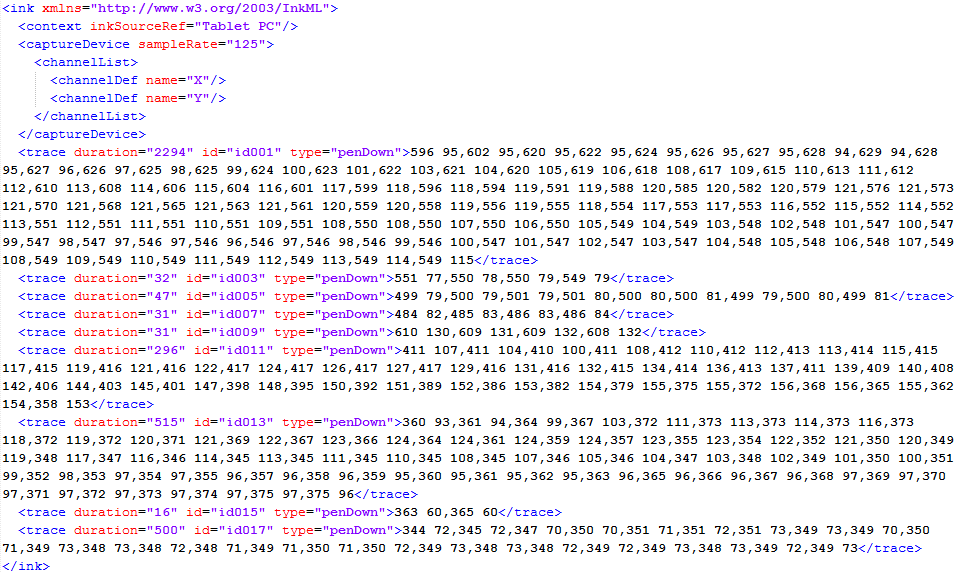
\includegraphics[width=1\textwidth]{./figures/adab_inkml}
\caption{Trajectory information of a city name sample.}
\label{fig:adab_inkml}
\end{figure}

\begin{figure}
\centering
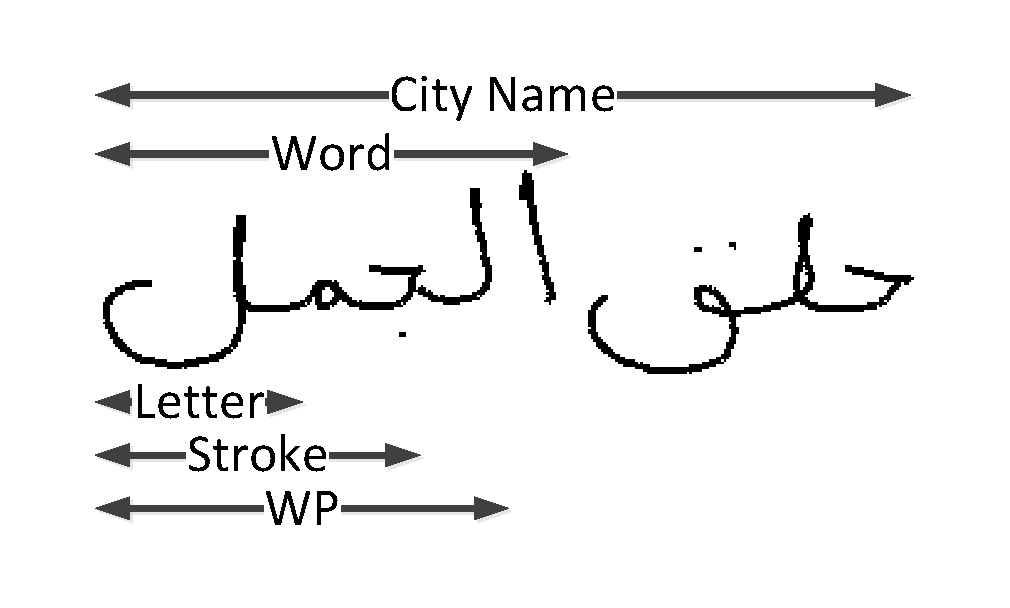
\includegraphics[width=0.4\textwidth]{./figures/sample_parts}
\caption{Visual demonstration of a test sample parts.}
\label{fig:sample_parts}
\end{figure}

%%%%%%%%%%%%%%%%%%%%%%%%%%%%%%%%%%%%%%%%%%%%%%%%%%%%%%%
\newpage{}
%%%%%%%%%%%%%%%%%%%%%%%%%%%%%%%%%%%%%%%%%%%%%%%%%%%%%%%

\section{Letter Samples Extraction}
\label{sec:letters_extraction}

\iftoggle{edit-mode}{\hspace{0pt}\marginpar{The missing information}}{}
The goal of this stage was to create a sufficiently large database of handwritten Arabic letters to be used by the letter classifier described in Chapter \ref{chap:classification}, and as a ground-truth for validating the segmentation method described in Chapter \ref{chap:segmentation}.
The absence of mapping between the strokes and letters in the ADAB database, required manual segmentation of the strokes trajectories.

\iftoggle{edit-mode}{\hspace{0pt}\marginpar{Letters extraction method}}{}
To facilitate the database construction, we have created a user friendly system that reads the samples from the ADAB database, displays the different strokes of a sample in different color, and enables a human expert to easily mark the segmentation points on the strokes.
Once the segmentation process is done, the match between the sub-strokes and the letters is performed in a semi-automatic manner, which required the expert intervention only in cases of ambiguity.  
The system was designed also to handle samples that included more than a single letter. 
In this case, the expert also had to relate the strokes to the different words.
The graphical user interface of the system is shown in Figure \ref{fig:manual_segmentation}. 

\begin{figure}[h]
\centering
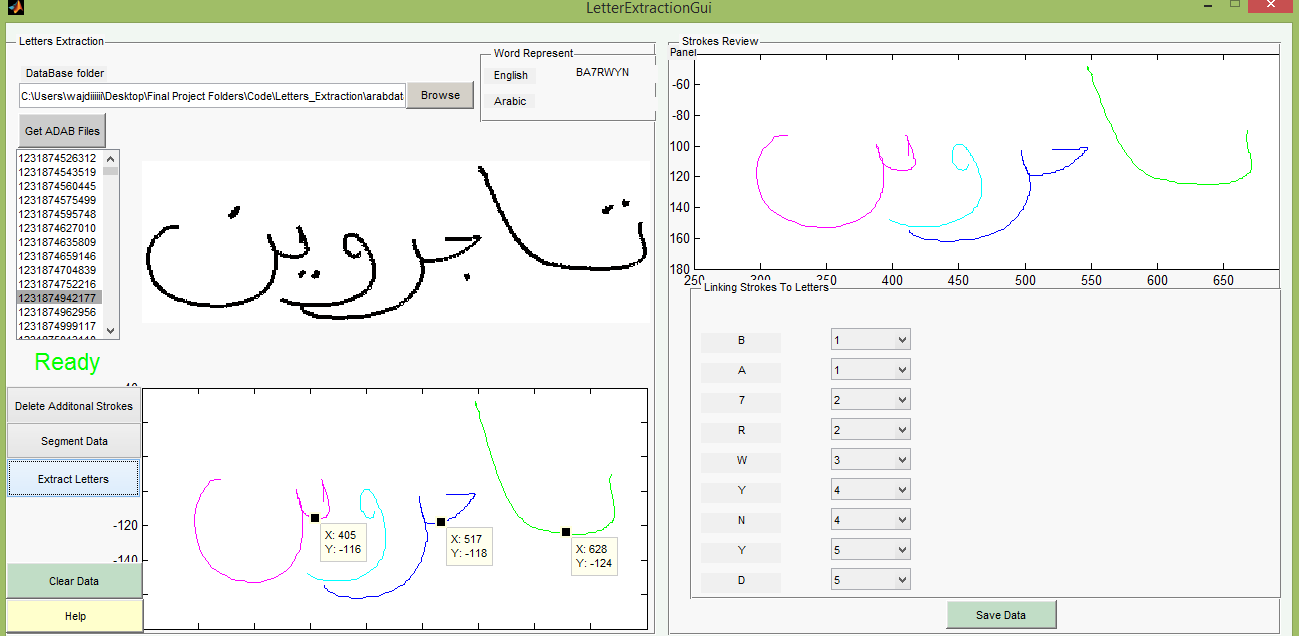
\includegraphics[width=1\textwidth]{./figures/manual_segmentation}
\caption{A view of manual segmentation system.}
\label{fig:manual_segmentation}
\end{figure}

\iftoggle{edit-mode}{\hspace{0pt}\marginpar{Additional strokes detection and removal}}{}
Since, neither the classification system nor the segmentation process consider the additional strokes, the system automatically filtered them out. 
The detection of delayed strokes was performed based on the stroke size and the area of its bounding box. 
However, in order to avoid unintentionally removing main bodies of small letters, we set a relatively high threshold.
Thus, the human expert had to filter out additional strokes manually that could not be identified by the system as such.

\iftoggle{edit-mode}{\hspace{0pt}\marginpar{The output structure}}{}
The output of the system was saved in a parsed XML file for each sample. 
As can be seen in Figure \ref{fig:adab_segmented_xml}, the hierarchy of the out XML represents the structure of the sample as defined in Figure \ref{fig:sample_parts}. 
In order to build up the letters database, an automatic procedure was implemented to extract the letters trajectories from the output XML. 
The letters database consists of directories that represent the different letters.
Each letter directory contains four folders, named Iso, Mid, Fin and Iso which contains the corresponding letter samples, recorded in a Matlab data files.
In the case of a dis-connective letter, the letter folder contains two directories representing the Iso and Mid forms of the corresponding letter.
For the sake of obtaining a sample-set sufficiently large to be used for both learning and validation, more than 7k samples were manually segmented which consisted of about 20k letters. 

\begin{figure}
\centering
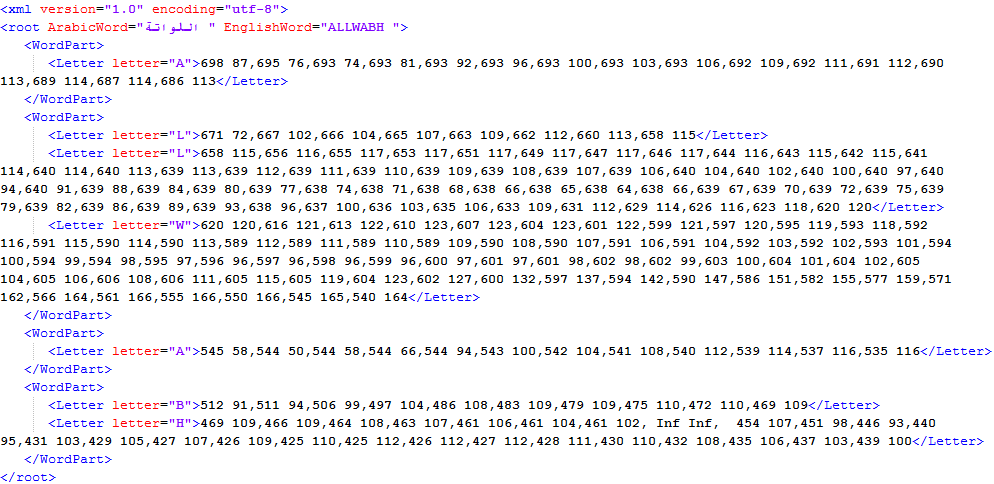
\includegraphics[width=1\textwidth]{./figures/adab_segmented_xml}
\caption{The output parsed  XML.}
\label{fig:adab_segmented_xml}
\end{figure}

%\bibliographystyle{plainnat}
%\bibliography{references}
%\end{document}

%\begin{itemize}
%\item mention that the number of samples per class is different from letter to letter
%\item see "Removing delayed strokes" section in \cite{jaeger2001online}
%\end{itemize}
